\section{Attack Trees}

Modifizierbare \textit{draw.io}-Datei 	
\href{https://mega.nz/file/qtgjgJ6C#xQwsQRziICS2bSHczp7AsqlcOLmHHHx8GFPwZvlDFkg}
{hier} downloaden zur näheren Inspizierung.\\

\begin{figure}[hbt!]
	\centering
		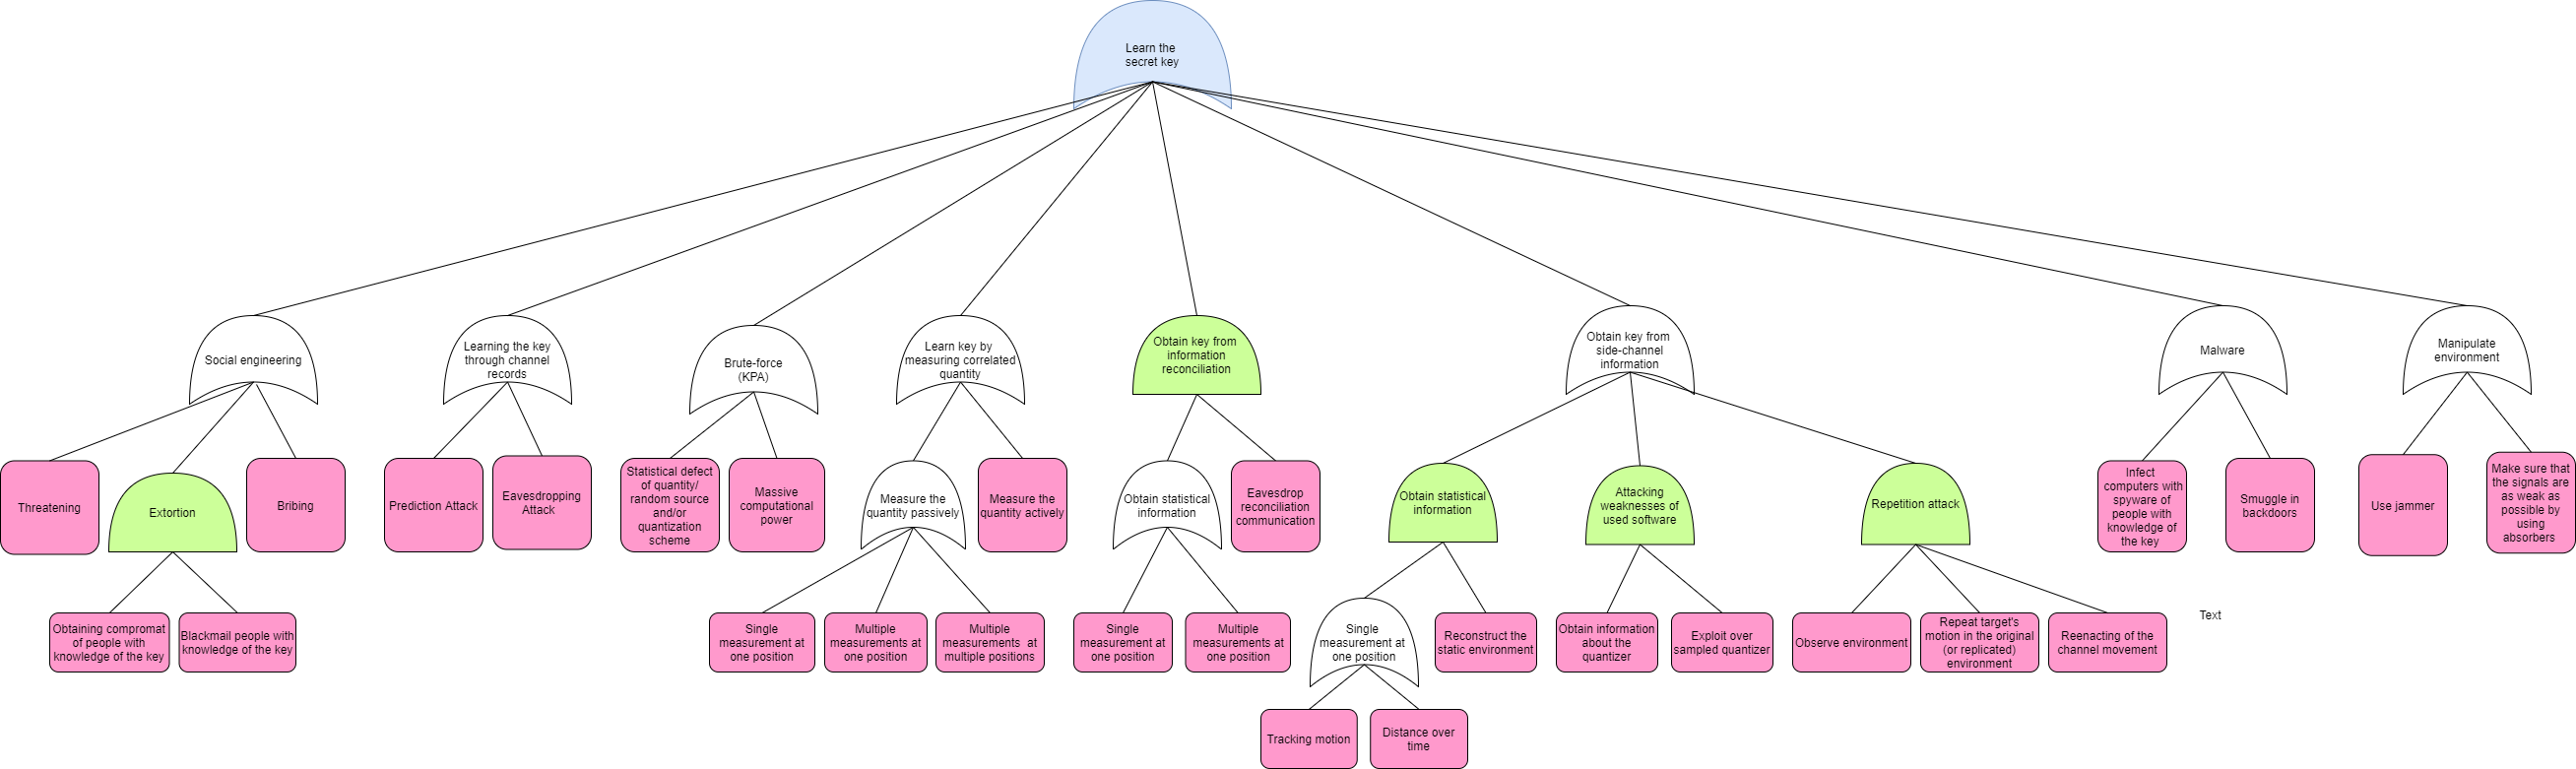
\includegraphics[width=1\textwidth ]
		{Bilder/a3-tree.png}
		\caption{Attack tree}
		\label{fig:3.1}
\end{figure}


Weitere Angriffsszenarien neben 
\begin{itemize}
	\item \textit{Repetition Attack}
	\item \textit{Prediction Attack}
	\item \textit{Eavesdropping Attack}
	\item \textit{Angriff auf den Quantisierer}\\[0.6mm]
\end{itemize}

sind unter anderem \textit{social engineering} Attacken
wie 

\begin{itemize}
	\item \textit{Bestechen}
	\item \textit{Drohen}
	\item \textit{Erpressen mithilfe von 
	Kompromat}\\[0.6mm]
\end{itemize}

oder \textit{Schadsoftwareattacken}
wie 
\begin{itemize}
	\item Spyware
	\item Backdoors\\[0.6mm]
\end{itemize}

sowie \textit{Manipulation des Kanals} wie

\begin{itemize}
	\item Jammen
	\item Signalabsorber
	\item Attacken wie das Alternieren zwischen Umklammern 
	und Loslassen der Antenne\\[0.6mm]
\end{itemize}